\documentclass[12pt,letterpaper]{article}
\usepackage{amsmath,amsthm,amsfonts,amssymb,amscd}
\usepackage{fullpage}
\usepackage{lastpage}
\usepackage{enumerate}
\usepackage{fancyhdr}
\usepackage{mathrsfs}
\usepackage[margin=3cm,bottom=6cm]{geometry}
\usepackage{wrapfig}
\usepackage{graphicx}

\setlength{\parindent}{0.0in}
\setlength{\parskip}{0.05in}

\renewcommand{\theenumi}{\bf\Alph{enumi}}


% Edit these as appropriate
\newcommand\course{Math 227C}
%\newcommand\semester{Spring 2019}     % <-- current semester
\newcommand\hwnum{1}                  % <-- homework number
\newcommand\yourname{Jun Allard} % <-- your name
%\newcommand\login{jcarberr}           % <-- your CS login

\newenvironment{answer}[1]{
  \subsubsection*{Problem \hwnum.#1}
}{\newpage}

\pagestyle{fancyplain}
\headheight 35pt
\lhead{ \course\ }
\chead{\textbf{ Problem Set 1 }}
%\rhead{Due {\bf Friday, April 13th}}
\headsep 20pt

\begin{document}


\begin{enumerate}[A.]

%%%%%%%%%%%%%% PROBLEM %%%%%%%%%%%%%%%%%%
\item Two fair dice are rolled, one after the other.
\begin{enumerate}[i.]
\item Let $E_{6}$ be the event that the sum of the dice is 6. Let $F_4$ be the event that the first die is 4. Are these two events independent?
\item Let $E_{7}$ be the event that the sum of the dice is 7. Let $F_4$ be the event that the first die is 4. Are these two events independent?
\item Let $E_i$ be the event that the sum of the dice is $i$. Let $F_j$ be the event that the first die is $j$. For what values of $i$ and $j$ are these two events independent?
\end{enumerate}

%%%%%%%%%%%%%% PROBLEM %%%%%%%%%%%%%%%%%%
\item Consider a simple protein-protein interaction network with a receptor, five proteins numbers 1 to 5, and a gene promotor.
You have determined that the proteins interact according to the figure below. 
In a population of cells, you find that each protein has a probability $p_i$ of being functionally active in a given cell, where $i=1,2,3,4,5$. 
\begin{figure}[h!]
\centering
\centering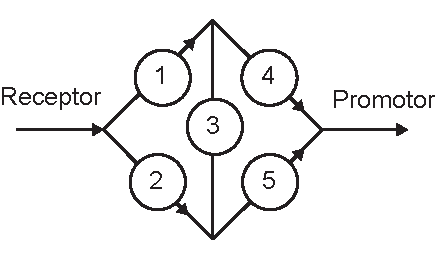
\includegraphics[width=8cm]{figP12}
\end{figure}
A functional signal transduction requires at least one complete path from the membrane receptor (R) to the transcription factor (TF). 
Protein P3 can interact bidirectionally with both P2 and P4 (acting as a scaffold protein). 
Assume that the proteins are active independently of each other.
Calculate the probability that signal transduction occurs successfully in this network.

\end{enumerate}

\end{document}
